\chapter{Seznam použitých zkratek}
\renewcommand{\glossarysection}[2][]{}
\printglossary[type=acronym]
% \printglossaries



% \chapter{UML diagramy}
% \textbf{\large Tato příloha není povinná a zřejmě se neobjeví v každé práci. Máte-li ale větší množství podobných diagramů popisujících systém, není nutné všechny umísťovat do hlavního textu, zvláště pokud by to snižovalo jeho čitelnost.}



\chapter{Instalační a uživatelská příručka}
% \section{Nároky aplikace}
% Aplikace je plně funkční v každém webovém prohlížeči dodržujícím specifikace \emph{XHTML Mobile Profile 1.1} \cite{XhtmlMpDoc}, \emph{ECMAScript Mobile Profile 1.0} \cite{EsMpDoc}, \emph{CSS 2.1} \cite{CssDoc} a \emph{PNG W3C/ISO/IEC version} \cite{PngDoc}, přesto je ale pravděpodobné, že bude fungovat, byť třeba omezeně, i v jiných prohlížečích.
% 
% \section{Instalace aplikace}
% Celý adresář s aplikací nahrajte do požadovaného umístění.\footnote{Při volbě umístění berte ohled na prostředí, do kterého aplikaci nahráváte. Mnoho mobilních telefonů má pro HTML stránky, které aplikaci tvoří, vyhrazené umístění.} Tím je aplikace nainstalována a připravena k použití.
% 
% \section{Spuštění aplikace}
% Aplikaci spustíte otevřením souboru \emph{index.html}, který se nachází v adresáři s aplikací, prostřednictvím internetového prohlížeče.\footnote{V mobilním prostředí například mobilní verze prohlížečů Opera, NetFront, Safari, Nokia Mini Map, Firefox, Internet Explorer...}\footnote{Pokud používáte prohlížeč Opera Mobile a nemáte v něm dialog pro otevření lokálního souboru, zadejte do adresního řádku protokol \emph{file://}, potvrďte a dialog se zobrazí.}
% 
% \section{Možnosti vyhledávání}
% Hledanou místnost můžete zadat do vyhledávacího pole aplikace jako:
% \begin{itemize}
%  \item jméno místnosti (např. KN:E-107),
%  \item jméno místnosti před přečíslováním v roce 2008 (např. K1),
%  \item zažité pojmenování místnosti (např. Zengerova posluchárna),
%  \item jméno sídlícího vyučujícího (např. Josef Vomáčka).
% \end{itemize}
% Zadat lze i část názvu hledaného umístění, při vyhledávání se nerozlišuje velikost písmen a~lze použít ECMAScriptové regulární výrazy, k nimž je návod v aplikaci a specifikace na~\cite{EsReDoc}.
% 
% \subsection{Hledání v okolí}
% Aplikace umožňuje vyhledávání bodů zájmu (občerstvení, výtahy, toalety...) v okolí místnosti. Vyhledejte běžným způsobem místnost a na plánku se v jejím okolí mimo ní zobrazí i~body zájmu.
% 
% \subsection*{Přímo v aplikaci je k dispozici nápověda.}



\chapter{Obsah přiloženého CD}
% \textbf{\large Tato příloha je povinná pro každou práci. Každá práce musí totiž obsahovat přiložené CD. Viz dále.}
% 
% Může vypadat například takto. Váš seznam samozřejmě bude odpovídat typu vaší práce. (viz \cite{infodp}):
% 
% \begin{figure}[h]
% \begin{center}
% \includegraphics[width=14cm]{figures/seznamcd}
% \caption{Seznam přiloženého CD --- příklad}
% \label{fig:seznamcd}
% \end{center}
% \end{figure}
% 
% Na GNU/Linuxu si strukturu přiloženého CD můžete snadno vyrobit příkazem:\\ 
% \verb|$ tree . >tree.txt|\\
% Ve vzniklém souboru pak stačí pouze doplnit komentáře.
% 
% Z \textbf{README.TXT} (případne index.html apod.)  musí být rovněž zřejmé, jak programy instalovat, spouštět a jaké požadavky mají tyto programy na hardware.
% 
% Adresář \textbf{text}  musí obsahovat soubor s vlastním textem práce v PDF nebo PS formátu, který bude později použit pro prezentaci diplomové práce na WWW.

% Obsah přiloženého CD je zobrazený na obrázku \ref{fig:tree}.
% \begin{figure}[ht]
% \begin{center}
% 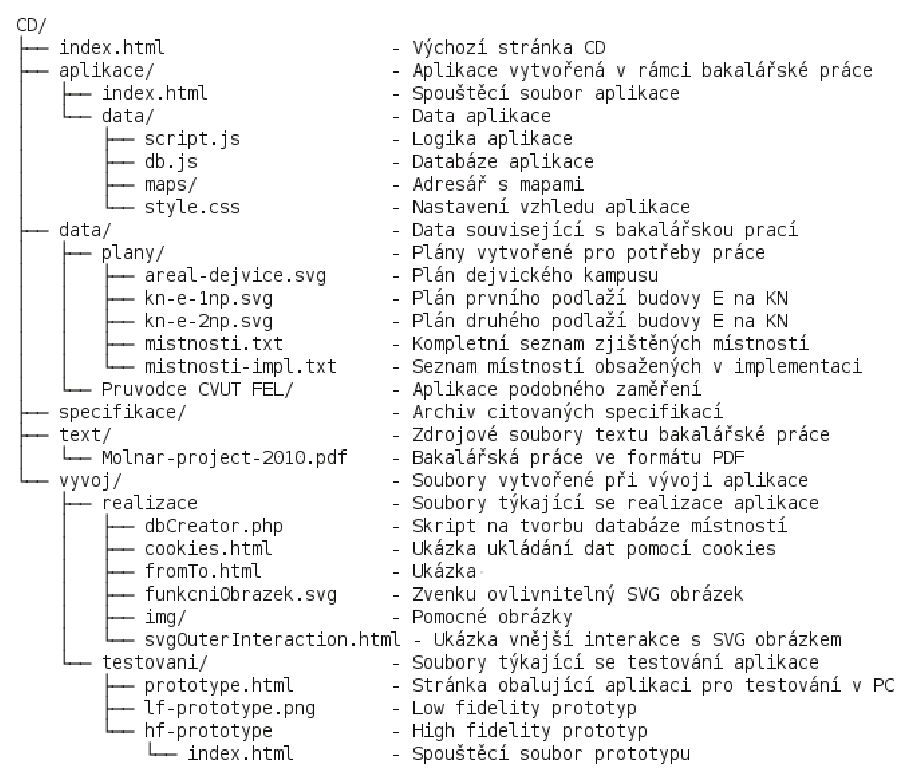
\includegraphics{figures/tree}
% % \caption{Struktura přiloženého CD}
% % \label{fig:tree}
% \end{center}
% \end{figure}

% $\vdash──$ \texttt{date-utils@1.2.10} -- popisek \\
% $\vdash─\top$ \texttt{express@2.5.6} \\
% $\mid \vdash─\top$ \texttt{connect@1.8.5} \\
% $\mid \mid └──$ \texttt{formidable@1.0.8} \\
% $\mid \vdash──$ \texttt{mime@1.2.4} \\
% $\mid \vdash──$ \texttt{mkdirp@0.0.7} \\
% $\mid └──$ \texttt{qs@0.4.1} \\
% $\vdash──$ \texttt{icalendar@0.4.1} \\
% $\vdash──$ \texttt{iconv@1.1.3} \\
% $\vdash─\top$ \texttt{jquery@1.6.3} \\
% $\mid \vdash──$ \texttt{htmlparser@1.7.4} \\
% $\mid └─\top$ \texttt{jsdom@0.2.10} \\
% $\mid   \vdash──$ \texttt{contextify@0.0.7} \\
% $\mid   \vdash──$ \texttt{cssom@0.2.2} \\
% $\mid   └──$ \texttt{request@2.9.100} \\
% $\vdash─\top$ \texttt{rdfstore@0.6.2} \\
% $\mid └──$ \texttt{mongodb@0.9.9-5} \\
% $└─\top$ \texttt{soap@0.1.2} \\
% $  \vdash──$ \texttt{node-expat@1.4.4/ \\
% $  └──$ \texttt{request@2.2.6} \\
% ├── date-utils@1.2.10 
% ├─┬ express@2.5.6 
% │ ├─┬ connect@1.8.5 
% │ │ └── formidable@1.0.8 
% │ ├── mime@1.2.4 
% │ ├── mkdirp@0.0.7 
% │ └── qs@0.4.1 
% ├── icalendar@0.4.1 
% ├── iconv@1.1.3 
% ├─┬ jquery@1.6.3 
% │ ├── htmlparser@1.7.4 
% │ └─┬ jsdom@0.2.10 
% │   ├── contextify@0.0.7 
% │   ├── cssom@0.2.2 
% │   └── request@2.9.100 
% ├─┬ rdfstore@0.6.2 
% │ └── mongodb@0.9.9-5 
% └─┬ soap@0.1.2 
%   ├── node-expat@1.4.4 
%   └── request@2.2.6 



\chapter{TODO}
\renewcommand*{\glspostdescription}{}
\printglossary[type=todo]
\noindent (Shodné položky jsou vynechány.)
